%%%%%%%%%%%%%%%%%%%%%%%%%%%%%%%%%%%%%%%%%%%%%%%%%%%%%%%%%%%%%%%%%%%%%%%%%%%%%%%%
% Template for USENIX papers.
%
% History:
%
% - TEMPLATE for Usenix papers, specifically to meet requirements of
%   USENIX '05. originally a template for producing IEEE-format
%   articles using LaTeX. written by Matthew Ward, CS Department,
%   Worcester Polytechnic Institute. adapted by David Beazley for his
%   excellent SWIG paper in Proceedings, Tcl 96. turned into a
%   smartass generic template by De Clarke, with thanks to both the
%   above pioneers. Use at your own risk. Complaints to /dev/null.
%   Make it two column with no page numbering, default is 10 point.
%
% - Munged by Fred Douglis <douglis@research.att.com> 10/97 to
%   separate the .sty file from the LaTeX source template, so that
%   people can more easily include the .sty file into an existing
%   document. Also changed to more closely follow the style guidelines
%   as represented by the Word sample file.
%
% - Note that since 2010, USENIX does not require endnotes. If you
%   want foot of page notes, don't include the endnotes package in the
%   usepackage command, below.
% - This version uses the latex2e styles, not the very ancient 2.09
%   stuff.
%
% - Updated July 2018: Text block size changed from 6.5" to 7"
%
% - Updated Dec 2018 for ATC'19:
%
%   * Revised text to pass HotCRP's auto-formatting check, with
%     hotcrp.settings.submission_form.body_font_size=10pt, and
%     hotcrp.settings.submission_form.line_height=12pt
%
%   * Switched from \endnote-s to \footnote-s to match Usenix's policy.
%
%   * \section* => \begin{abstract} ... \end{abstract}
%
%   * Make template self-contained in terms of bibtex entires, to allow
%     this file to be compiled. (And changing refs style to 'plain'.)
%
%   * Make template self-contained in terms of figures, to
%     allow this file to be compiled.
%
%   * Added packages for hyperref, embedding fonts, and improving
%     appearance.
%
%   * Removed outdated text.
%
%%%%%%%%%%%%%%%%%%%%%%%%%%%%%%%%%%%%%%%%%%%%%%%%%%%%%%%%%%%%%%%%%%%%%%%%%%%%%%%%

\documentclass[letterpaper,twocolumn,10pt]{article}
\usepackage{usenix2019_v3}

% to be able to draw some self-contained figs
\usepackage{tikz}
\usepackage{amsmath}

\begin{document}

%don't want date printed
\date{}

% make title bold and 14 pt font (Latex default is non-bold, 16 pt)
\title{\Large \bf Extending a File System to Support NVMe Devices Using SPDK}

%for single author (just remove % characters)
\author{
{\rm Ao Li}\\
University of Toronto
\and
{\rm Geoffrey Yu}\\
University of Toronto
} % end author

\maketitle

\begin{abstract}
Non-volatile memory express (NVMe) based solid state devices have undergone
tremendous innovation---leading to significant increases in performance.
However file systems have been slow to keep up; in many cases their design
(kernel space and lock based) impedes their ability to leverage the full
performance offered by NVMe storage devices. So how should next generation file
systems be designed to leverage the performance offered by NVMe storage
devices?

In this work we take a first step towards answering this question by extending
an existing user space file system to support NVMe storage devices by using
SPDK---a user space, polled, lockless device driver. We additionally modify 
the write path of the file system to support multi-threaded asynchronous I/O. The key
idea behind our design is to use a multi-threaded architecture to be able to
submit asynchronous I/O requests for different types of file system blocks
(e.g.  metadata versus data) in parallel.

Through experiments, we show that our multi-threaded asynchronous write
path is able to offer up to a $1.5\times$ improvement for single file writes
and up to a $3\times$ improvement for multi-file single transaction writes when
compared to a write path implemented with synchronous I/O.
\end{abstract}

\section{Introduction}
The emergence of the non-volatile memory express (NVMe)
specification~\cite{nvme} coupled with faster solid state storage devices
(SSDs) have together paved the way for new opportunities to improve the
performance of storage applications. In particular, the NVMe specification
introduces new avenues for parallelism by providing applications parallel
access to the underlying storage device through multiple I/O
queues~\cite{nvme}. File systems, a major storage application, are prime
candidates for these performance improvement opportunities.

Unfortunately, many file systems today are not designed to take advantage of
these opportunities. They
\begin{enumerate*}[label={(\roman*)}]
  \item reside in kernel space, requiring slow context switches to access;
  \item use locks to coordinate access to shared data, limiting their
    scalability; and
  \item are not written to take advantage of the parallelism exposed by NVMe.
\end{enumerate*}
So how should next generation file systems be designed to leverage the
performance improvements offered by NVMe storage devices?

In this work we take a first step towards answering this question by extending
an existing user space file system to support NVMe storage devices. We do this
with the goal of {\it quantifying} the potential performance benefit of
NVMe-designed file systems. Specifically, as a proof of concept, we integrate
testFS~\cite{testfs} (a toy user space file system) with SPDK~\cite{spdk} (a
user space lockless driver for NVMe devices) and we modify the file system's
write path to support multi-threaded asynchronous I/O.

The key idea in our design is to use a multi-threaded architecture to allow
different types of I/O requests to be submitted to and queued on the storage
device in parallel. This approach enables us to improve the performance of the
file system's write path by submitting asynchronous I/O requests for file
system metadata (e.g. inodes) and data in parallel by using different threads.

We benchmark our implementation and show that it can offer up to a $1.5\times$
improvement on single file writes and up to a $3\times$ improvement on
multi-file single transaction writes when compared to synchronous I/O.

\vspace{0.75em}
\noindent
In summary, our project makes the following contributions:
\begin{itemize}
  \item We propose a method to support multi-threaded asynchronous I/O on an
    NVMe SSD that can be implemented alongside existing synchronous code.
  \item We implement a proof of concept of our design by modifying the testFS
    write path and integrating it with with SPDK.
  \item We benchmark our implementation and show that our design offers up to a
    $1.5\times$ improvement for single file writes and up to a $3\times$
    improvement for multi-file single transaction writes when compared to
    synchronous I/O.
\end{itemize}

\section{Background}

In this section we present the background of NVMe interface and SPDK 
framework. We also present testFS, a user space file system that our 
file system is based on.

\subsection{NVMe and I/O Queue}

NVMe~\cite{nvme} is an open interface specification designed to allow host
software to communicate with a non-volatile memory subsystem (NVM) via a 
peripheral component interconnect express (PCIe) bus. Previous standards
such as serial-attacked SCSI and serial advanced technology attachment
can handle queue depths of 254 and 32 respectively. NVMe is able to 
handle queue depths of up to 65535 I/O queues with up to 64 Ki outstanding
commands per I/O queue, which allows an NVMe device to support parallel
operations. An I/O queue is composed of a submission queue and a completion
queue. Host software issues I/O commands to a submission queue and completions
are placed into the associated completion queue by the controller. Note that
the order of completions is not determined by the submission oder of the commands.

\subsection{SPDK and Block Devices}

SPDK~\cite{spdk} is an open source library that allows developer to implement
high performance, scalable, user-mode storage applications. A block device 
in SPDK is an abstraction of all block devices, where I/O commands are 
processed and issued to corresponding physical block devices such as NVMe 
devices and Malloc devices. SPDK provides a event framework, where  
different threads to exchange data through passing messages to one another.
It allows a user to build asynchronous, lockless, and high performance
applications.

\begin{figure}
  \centering
  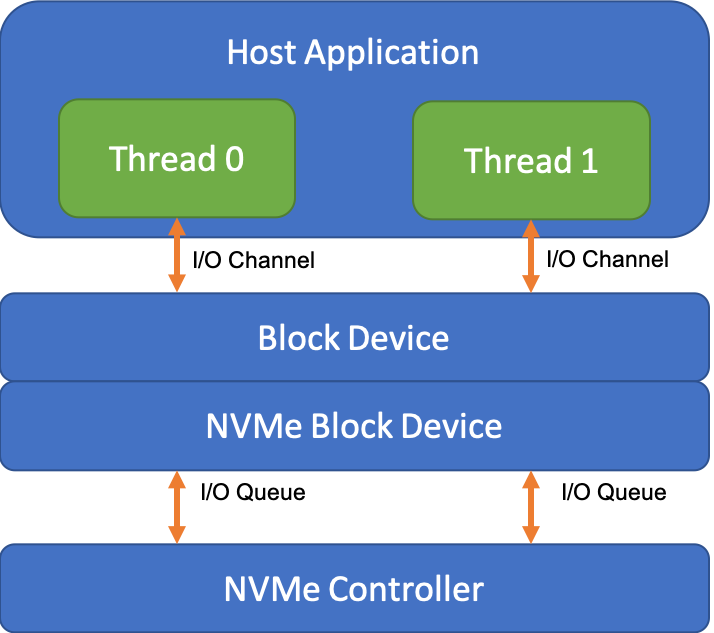
\includegraphics[height=6cm]{spdk_arch}
  \caption{Example of an SPDK application.}
  \label{fig:spdk_arch}
\end{figure}

For each thread, SPDK uses an io channel to represent the channel for accessing an 
I/O device. I/O requests issued to the block device will be forwarded to the underlying
physical device. In our implementation, io channel corresponds to I/O queue 
of the underlying NVMe device, the framework builds I/O commands based on I/O 
requests and submits them to submission queue. It then polls for I/O completion
on each queue pair with outstanding I/O to receive completion callbacks.  
Figure~\ref{fig:spdk_arch} provides a graphical
representation of a host application using SPDK block devices to interact with
an NVMe device. In the host application, each thread submit I/O requests to its
corresponding I/O channel and the I/O channel forward the I/O requests to the 
actual physical device based on the implementation of the physical block device.
The framework invokes the callback function when the I/O request is finished.

\subsection{TestFS}

TestFS\cite{testfs} is a user space file system which is similar to EXT3, a
journaled file system that is commonly used by the Linux kernel. TestFS
has three levels of indirections, which is illustrated in Figure~\ref{fig:testfs}.
A super block points to meta data and an inode block of the root directory. 
The meta data store the freemap of blocks as well as the checksum of the data blocks.
Inode blocks point to data blocks where the actual data are stored. In testFS, both 
directory data and indirect inode data are stored in data blocks. The
space for inode blocks and data blocks are pre-allocated and fixed during the
life cycle of testFS.

Note that our file system is based on testFS because testFS is well maintained, user
level, and well documented file system, that allows us to build a proof of concept
quickly. We believe our modifications to testFS can be applied to most of file systems.

\begin{figure}[h!]
  \centering
  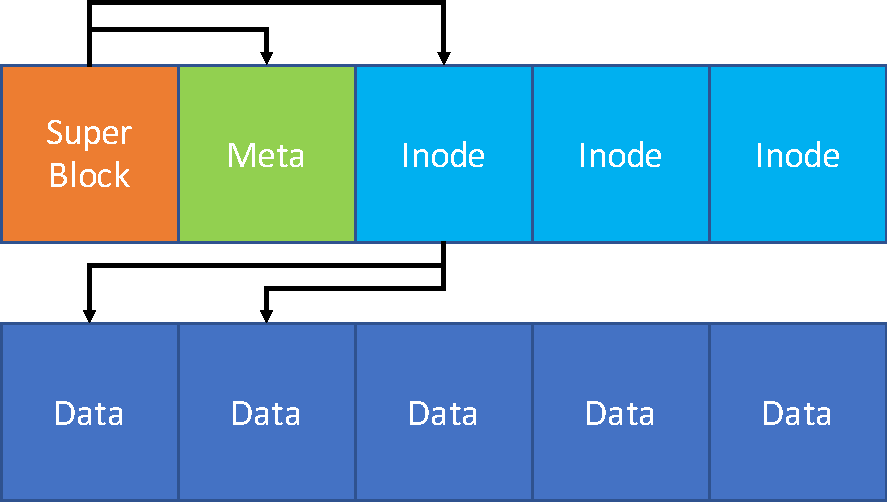
\includegraphics[height=3cm]{testfs}
  \caption{The layout of blocks with different types in testFS.}
  \label{fig:testfs}
\end{figure}

% TODO: Add more sections
\section*{Acknowledgments}
We would like to thank Shehbaz Jaffer for his guidance and feedback on our
project.


\bibliographystyle{plain}
\bibliography{report}

\end{document}
%%  LocalWords:  endnotes includegraphics fread ptr nobj noindent
%%  LocalWords:  pdflatex acks
